\documentclass[11pt]{article}

\usepackage{fancyhdr}
\usepackage{extramarks}
\usepackage{amsmath}
\usepackage{amsthm}
\usepackage{amsfonts}
\usepackage{tikz}
\usepackage{algorithmicx}
\usepackage{algpseudocode}
\usepackage{xcolor}
\usepackage{listings}
\usepackage{graphicx}
\usepackage{listings}
\usepackage{color}
\usepackage{xcolor}
\usepackage{float} 
\usepackage{subfig}
\usepackage[margin=1.5cm]{ geometry}

\definecolor{dkgreen}{rgb}{0,0.6,0}
\definecolor{gray}{rgb}{0.5,0.5,0.5}
\definecolor{mauve}{rgb}{0.58,0,0.82}
\lstset{frame=tb,
     language=Python,
     aboveskip=3mm,
     belowskip=3mm,
     showstringspaces=false,
     columns=flexible,
     basicstyle = \ttfamily\small,
     numbers=none,
     numberstyle=\tiny\color{gray},
     keywordstyle=\color{blue},
     commentstyle=\color{dkgreen},
     stringstyle=\color{mauve},
     breaklines=true,
     breakatwhitespace=true,
     tabsize=3
}
\usetikzlibrary{automata,positioning}

%
% Basic Document Settings
%

\topmargin=-0.45in
\evensidemargin=0in
\oddsidemargin=0in
\textwidth=6.5in

\textheight=9.0in
\headsep=0.25in

\linespread{1.}

\pagestyle{fancy}
\lhead{\hmwkAuthorName}
\chead{\hmwkClass\ (\hmwkClassInstructor\ \hmwkClassTime): \hmwkTitle}
\rhead{\firstxmark}
\lfoot{\lastxmark}
\cfoot{\thepage}

\renewcommand\headrulewidth{0.4pt}
\renewcommand\footrulewidth{0.4pt}
\renewcommand{\baselinestretch}{1.5}

\setlength\parindent{0pt}

\lstdefinestyle{lfonts}{ 
    basicstyle = \footnotesize\ttfamily, 
    stringstyle = \color{purple}, 
    keywordstyle = \color{blue!60!black}\bfseries, 
    commentstyle = \color{olive}\scshape, 
} 
\lstdefinestyle{lnumbers}{ 
    numbers = left, 
    numberstyle = \tiny, 
    numbersep = 1em, 
    firstnumber = 1, 
    stepnumber = 1, 
} 
\lstdefinestyle{llayout}{ 
    breaklines = true, 
    tabsize = 2, 
    columns = flexible, 
} 
\lstdefinestyle{lgeometry}{ 
    xleftmargin = 20pt, 
    xrightmargin = 0pt, 
    frame = tb, 
    framesep = \fboxsep, 
    framexleftmargin = 20pt, 
} 
\lstdefinestyle{lgeneral}{ 
    style = lfonts, 
    style = lnumbers, 
    style = llayout, 
    style = lgeometry, 
} 
\lstdefinestyle{python}{ 
    language = {Python}, 
    style = lgeneral, 
}

%
% Create Problem Sections
%

\newcommand{\enterProblemHeader}[1]{
    \nobreak\extramarks{}{Problem \arabic{#1} continued on next page\ldots}\nobreak{}
    \nobreak\extramarks{Problem \arabic{#1} (continued)}{Problem \arabic{#1} continued on next page\ldots}\nobreak{}
}

\newcommand{\exitProblemHeader}[1]{
    \nobreak\extramarks{Problem \arabic{#1} (continued)}{Problem \arabic{#1} continued on next page\ldots}\nobreak{}
    \stepcounter{#1}
    \nobreak\extramarks{Problem \arabic{#1}}{}\nobreak{}
}

\setcounter{secnumdepth}{0}
\newcounter{partCounter}
\newcounter{homeworkProblemCounter}
\setcounter{homeworkProblemCounter}{1}
\nobreak\extramarks{Problem \arabic{homeworkProblemCounter}}{}\nobreak{}

%
% Homework Problem Environment
%
% This environment takes an optional argument. When given, it will adjust the
% problem counter. This is useful for when the problems given for your
% assignment aren't sequential. See the last 3 problems of this template for an
% example.
%
\newenvironment{homeworkProblem}[1][-1]{
    \ifnum#1>0
        \setcounter{homeworkProblemCounter}{#1}
    \fi
    \section{Problem \arabic{homeworkProblemCounter}}
    \setcounter{partCounter}{1}
    \enterProblemHeader{homeworkProblemCounter}
}{
    \exitProblemHeader{homeworkProblemCounter}
}

%
% Homework Details
%   - Title
%   - Due date
%   - Class
%   - Section/Time
%   - Instructor
%   - Author
%

\newcommand{\hmwkTitle}{Assignment.\ \#2}
\newcommand{\hmwkDueDate}{Apr. 21, 2020}
\newcommand{\hmwkClass}{CSCI933}
\newcommand{\hmwkClassTime}{}
\newcommand{\hmwkClassInstructor}{Professor Chao Sun}
\newcommand{\hmwkAuthorName}{\textbf{Group}}

%
% Title Page
%

\title{
    \vspace{2in}
    \textmd{\textbf{\hmwkClass:\ \hmwkTitle}}\\
    \normalsize\vspace{0.1in}\small{Due\ on\ \hmwkDueDate\ at 10:00pm}\\
    \vspace{0.1in}\large{\textit{\hmwkClassInstructor\ \hmwkClassTime}}
    \vspace{3in}
}

\author{\hmwkAuthorName}
\date{}

\renewcommand{\part}[1]{\textbf{\large Part \Alph{partCounter}}\stepcounter{partCounter}\\}

%
% Various Helper Commands
%

% Useful for algorithms
\newcommand{\alg}[1]{\textsc{\bfseries \footnotesize #1}}

% For derivatives
\newcommand{\deriv}[1]{\frac{\mathrm{d}}{\mathrm{d}x} (#1)}

% For partial derivatives
\newcommand{\pderiv}[2]{\frac{\partial}{\partial #1} (#2)}

% Integral dx
\newcommand{\dx}{\mathrm{d}x}

% Alias for the Solution section header
\newcommand{\solution}{\textbf{\large Solution}}

% Probability commands: Expectation, Variance, Covariance, Bias
\newcommand{\E}{\mathrm{E}}
\newcommand{\Var}{\mathrm{Var}}
\newcommand{\Cov}{\mathrm{Cov}}
\newcommand{\Bias}{\mathrm{Bias}}

\begin{document}

\maketitle

\pagebreak

\section{1. Introduction}
The Pima are a group of Native Americans living in Arizona. A genetic predisposition allowed this group to survive normally to a diet poor of carbohydrates for years. In the recent years, because of a sudden shift from traditional agricultural crops to processed foods, together with a decline in physical activity, made them develop the highest prevalence of type 2 diabetes and for this reason they have been subject of many studies.\\
The type of dataset and problem is a classic supervised binary classification. Given a number of elements all with certain characteristics (features), we want to build a machine learning model to identify people affected by type 2 diabetes.\\
To solve the problem we will have to analyse the data, do any required transformation and normalisation, apply six machine learning algorithm GaussianNB, RandomForest, K Nearest Neighbour,Decision Tree,Logistic Regression and SVM. Here are some introduction:\\
\section{2. Data preparation}
Through figure \ref{f1} simple statistics, it can be found that the ratio between sick and not sick is 67:33.
\begin{figure}[H]
    \centering
    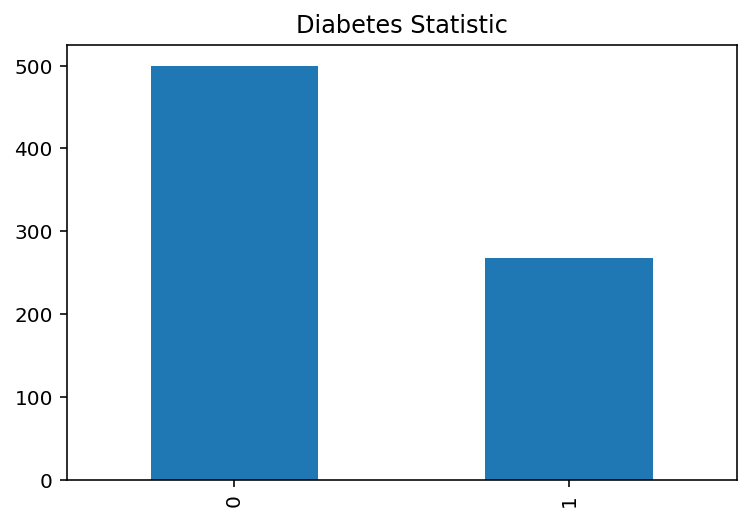
\includegraphics[width=0.6\textwidth]{ds}
    \caption{Diabetes Statistic}
    \label{f1}
\end{figure}

Then drawing histograms to visualize the data distribution of the eight features.
\begin{figure}[H]
    \centering
    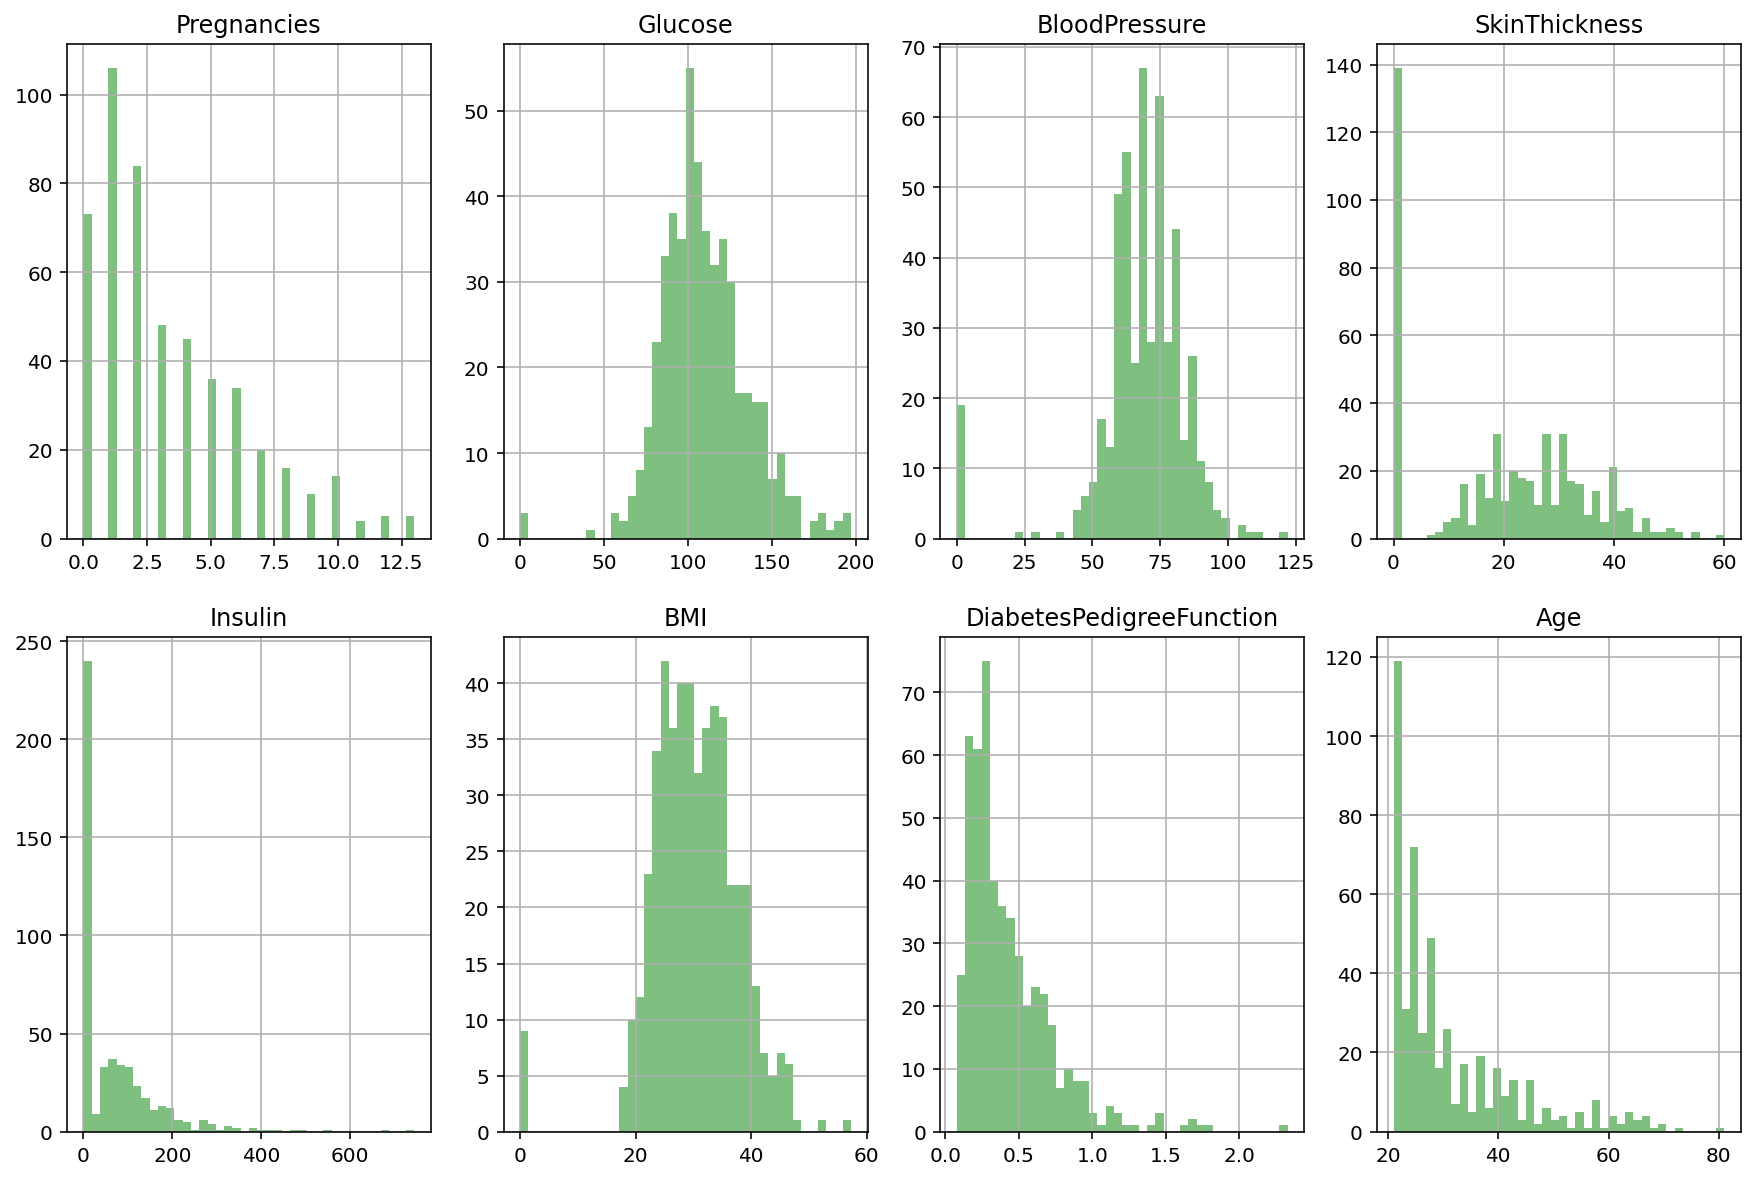
\includegraphics[width=0.8\textwidth]{h8}
    \caption{Features Distribution}
\end{figure}

It can be seen that there are some zero data, which may affect the accuracy of the training and affect the experimental results. Therefore, instead of directly removing the zero data, we chose to use the median to replace them, tere are the processed distribution:
\begin{figure}[H]
    \centering
    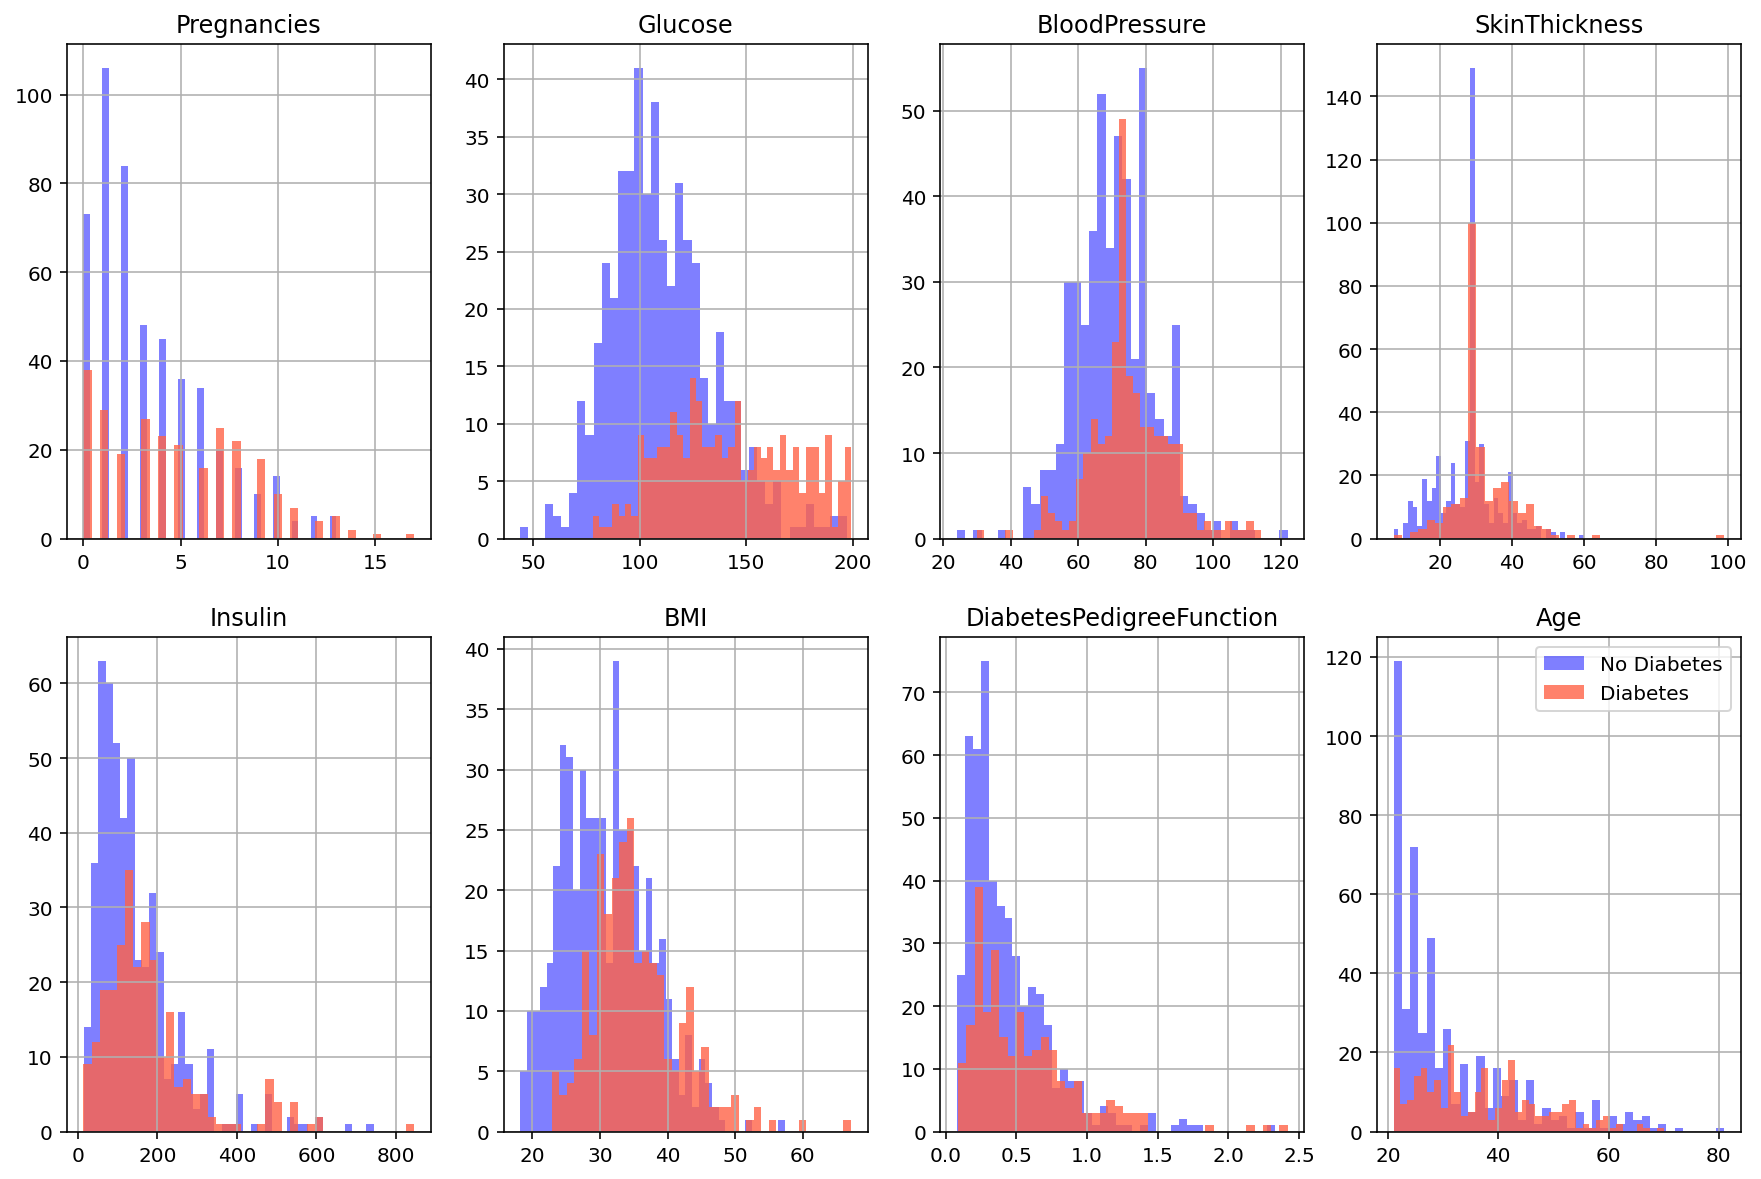
\includegraphics[width=0.8\textwidth]{h8opt}
    \caption{Features Processed Distribution}
\end{figure}

After that we split data to 80:20 for training and testing. In particular, because this is an imbalance dataset, adding stratify = y to ensure that the output of the split still maintains the same proportion of class 1 and 0. This is the end of Data preparation.



\section{3. Classifier}
\subsection{3.1 Logistic Regression}
A logistic regression model will be developed in an attempt to predict whether a patient is likely (represented by 1) or not likely (represented by 0) to develop diabetes in the next 5 years.
First, load the file to fetch the data, and split the data to the training set and test set by calling the function train\_test\_split. Besides, all the 8 characteristics are applied to trained the model. 
Once we have our training set and test set we can define a LogisticRegression model and fit it to our training data. Once trained, the model can then be used to make predictions against the test set.

\subsection{3.2 SVM}
A support vector machine (SVM) is a supervised machine learning model that uses classification algorithms for two-group classification problems.
\\
Suppose we are given a training dataset of $n$ points of the form,
\[
(x_1,y_1)...(x_n,y_n)
\]
where $y_i$ represents the classes, it is $-1$ or $1$.
\\
Any hyperplane can be written as the set of points $x_i$ satisfying:
\[
\omega*x_i-b=0
\]
By maximizing the distance between the planes, we could get a classifier to separate the data set.
\\
For the non-linear data set, it is suggested a way to create classifiers by applying the kernel trick. The idea is to classify non-linear data by cleverly mapping our space to a higher dimension. 
\\
Some common kernels include: Polynomial(we used in this project), Gaussian radial basis function and Hyperbolic tangent.
\\
Polynomial kernel function could be described by the equations:
\[
k*(x_i,x_j) = (x_i*x_i)^d
\]

\subsection{3.3 KNN}
The implementation of KNN is relatively simple: (1 Calculate the distance from the unknown instance to all known instances; (2 Select parameter K; (3 According to the majority-voting rule, classify unknown instances as the largest number of categories in the sample. n general, a larger K value during classification can reduce the impact of noise, but will blur the boundaries between categories. 
Therefore, the value of K is generally small (K < 20). The  measure of distance:
\[
d(x, y) = \sqrt{\sum^n_{i=0}(x_i-y_i)^2}
\]

\subsection{3.4 GaussianNB}
GaussianNB implements the Gaussian Naive Bayes classification algorithm, and this model assumes that the probability density function of all features conforms to a Gaussian distribution, whose the mean and variance of the distribution are estimated using maximum likelihood.
\[
P(x_i\lvert j) = \frac{1}{\sqrt{2\pi \sigma^2_y}} exp(- \frac{(x_i-\mu_y)^2}{2\sigma^2_y})
\]

\subsection{3.5 Decision Tree}
Decision tree learning uses a top-down recursive method, and its basic idea is to construct a tree with the fastest decrease in entropy value using information entropy as a measure.\\
Feature selection means that one feature is selected from the many features as the criterion of the current node split. There are different quantitative evaluation methods for the selected feature, so as to derive different decision trees. According to the selected feature evaluation criteria, the child nodes are generated recursively from top to bottom, and the decision tree stops growing until the data set is inseparable. Decision trees are easy to overfit and generally require pruning to reduce the size of the tree structure and alleviate overfitting

\subsection{3.5 RandomForest}
Standard Random Forest (RF) is based on decision tree as a basic learner, an extended algorithm based on Bagging, which adds random attribute selection in each round of decision tree training. 
when training in RF, for each node of the decision tree, the entire attribute set from the current node 
Randomly select a subset containing k attributes, and then select an optimal partition attribute from this subset. Usually choosing k as:
\[
k = \log^d_2 \;or\; k = \log^d_2 + 1
\]\\

This is the result based on the above classifier(See the code attachment for the specific implementation process).

\begin{figure}[H]
    \centering
    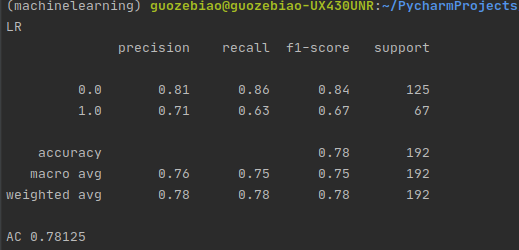
\includegraphics[width=0.6\textwidth]{lg}
    \caption{Logistic Regression}
\end{figure}

\begin{figure}[H]
    \centering
    \subfloat{
        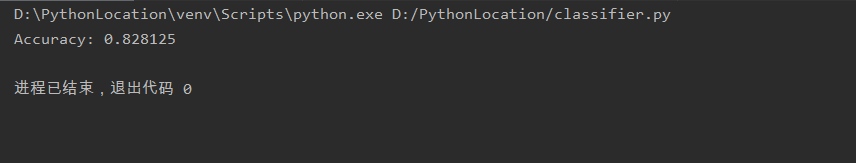
\includegraphics[width=0.4\textwidth]{dt}}
    \subfloat{
        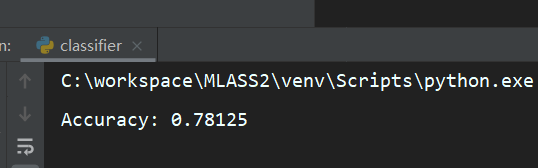
\includegraphics[width=0.4\textwidth]{svm}}
    \caption{DT vs SVM}
\end{figure}

\begin{figure}[H]
    \centering
    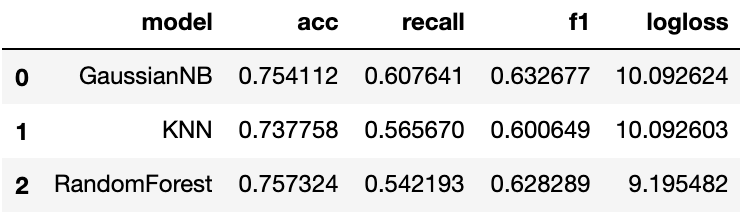
\includegraphics[width=1\textwidth]{three}
    \caption{GNB vs KNN vs RFC}
\end{figure}


\section{4.Evaluation}
Through the adjustment and optimization of superparameters and thresholds, three classifiers are left behind.\\
At the same time, from Figure \ref{f1} considering that this is a imbalance dataset set, the accuracy rate is not a good evaluation model, so we use the Recall rate to evaluate, while considering loss and time consumed.

\begin{figure}[H]
    \centering
    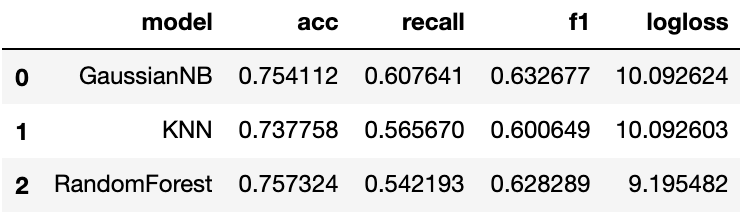
\includegraphics[width=1\textwidth]{three}
    \caption{Baeline Models}
\end{figure}

\begin{figure}[H]
    \centering
    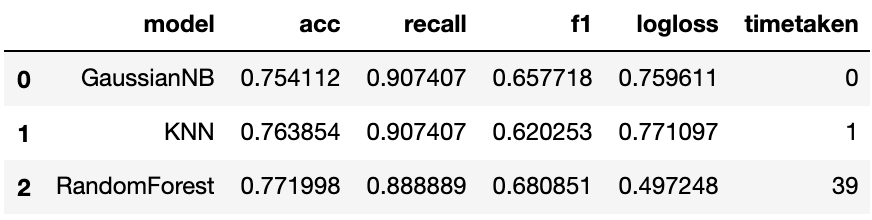
\includegraphics[width=1\textwidth]{threeopt}
    \caption{Optimal Models}
\end{figure}

\begin{figure}[H]
    \centering
    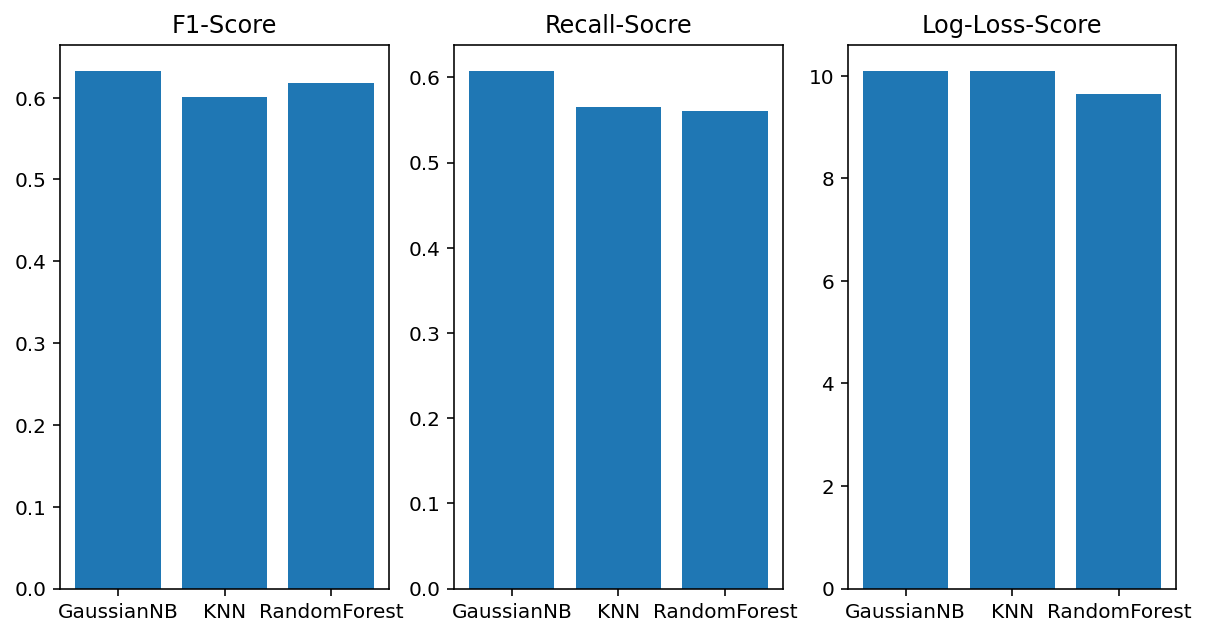
\includegraphics[width=0.8\textwidth]{br}
    \caption{Baseline Record}
\end{figure}

\begin{figure}[H]
    \centering
    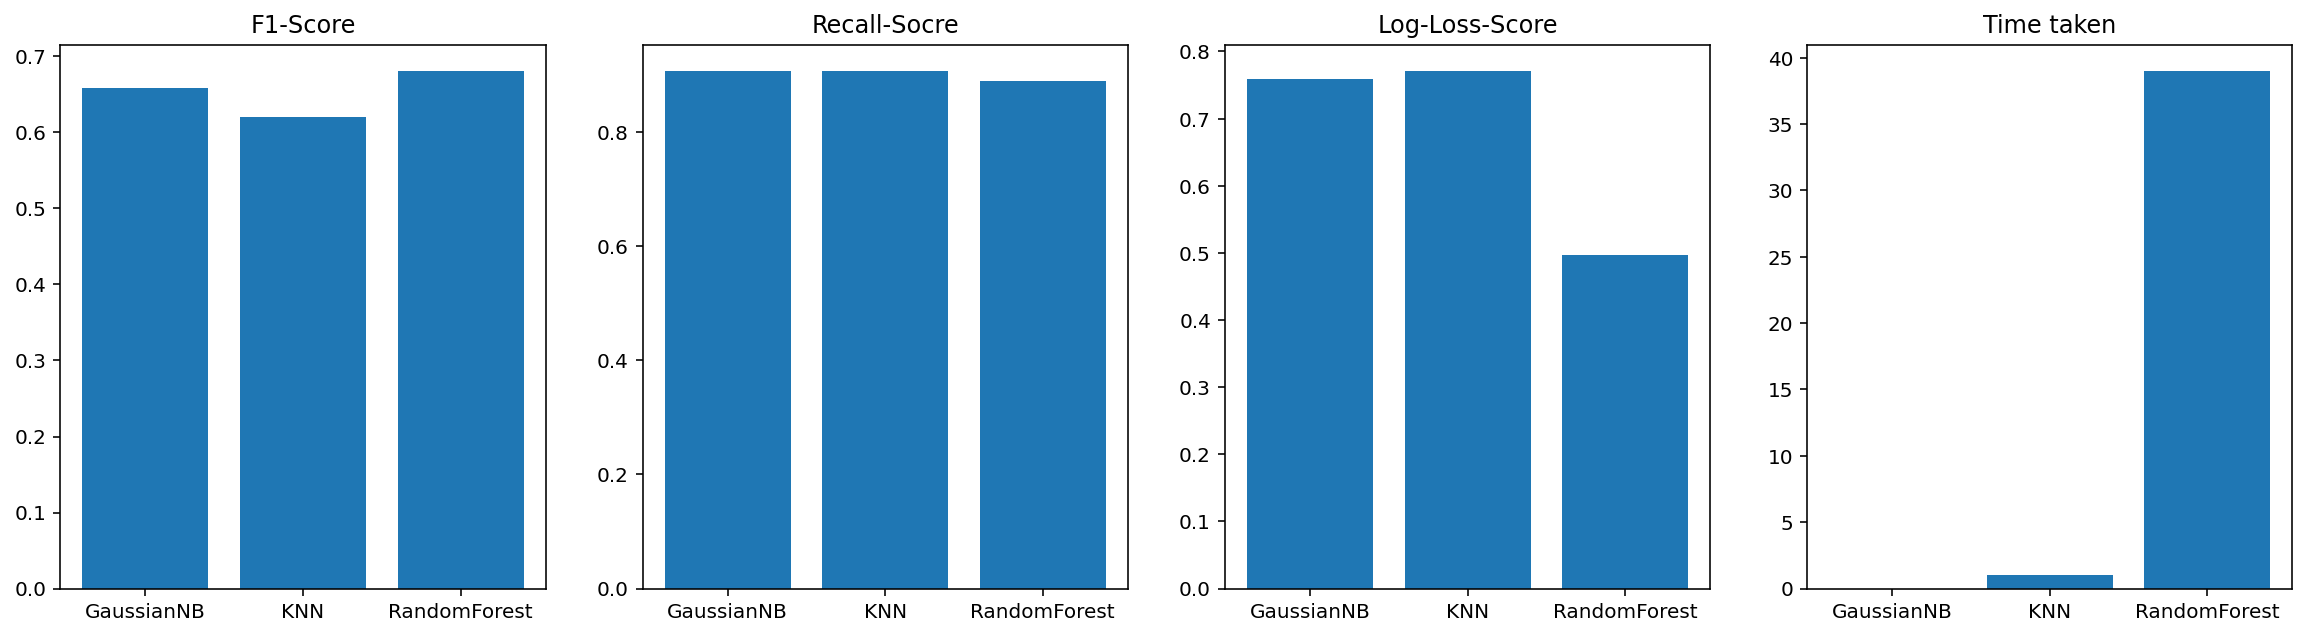
\includegraphics[width=1\textwidth]{or}
    \caption{Optimal Record}
\end{figure}


\section{5.Conclusions}
Although RandomForest can achieve good F1-Score and low loss, it consumes too much time. So from the comprehensive evaluation results, GaussianNB can achieve great results.\\
By GaussianNB classification, it also has better support for top feature.
\begin{figure}[H]
    \centering
    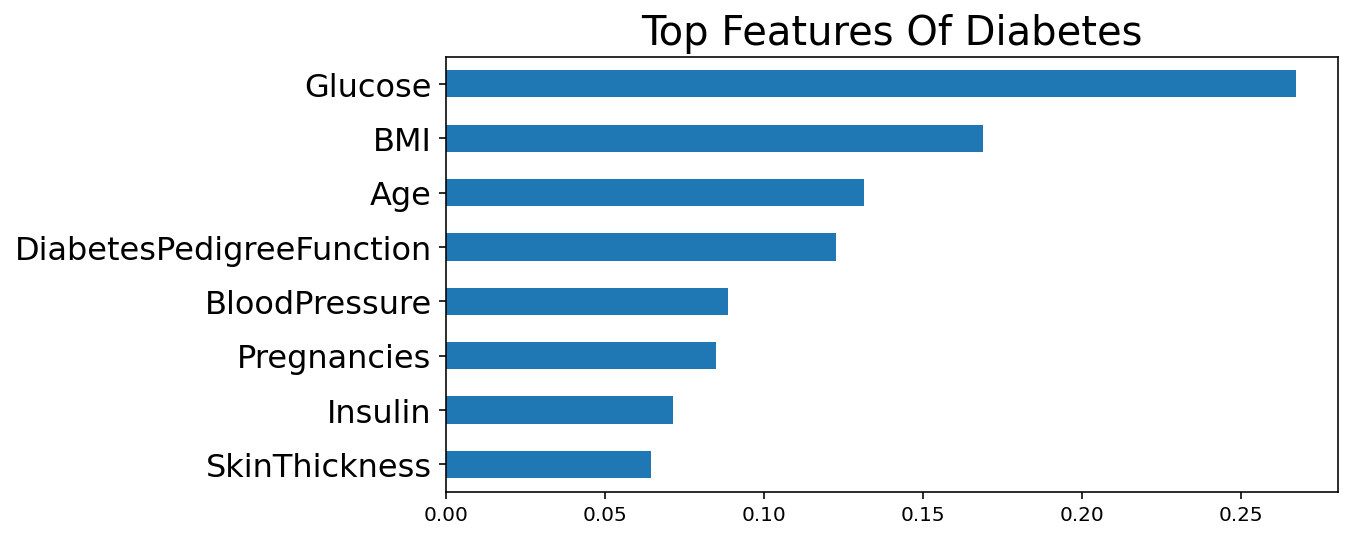
\includegraphics[width=1\textwidth]{tpf}
    \caption{Top Features}
\end{figure}

So, we can judge subgroup of Glucose and BMI that are more likely to have diabetes.

\section{6. Individual Effort}
Yao Xiao-2019180015: 30\% \\
Ruochen Liu-2019180018: 25\% \\
Zebiao Guo-2019180020: 25\% \\
Jun Wu-2019180006: 20\% \\
\end{document}
